% Figure -- the two molecular domains (small molecule vs protein backbone).
% \input{} from Ch2 (sec:molecular-domains). Source: figures/scripts/fig_ch2_domains.py
\begin{figure}[tbp]
\centering
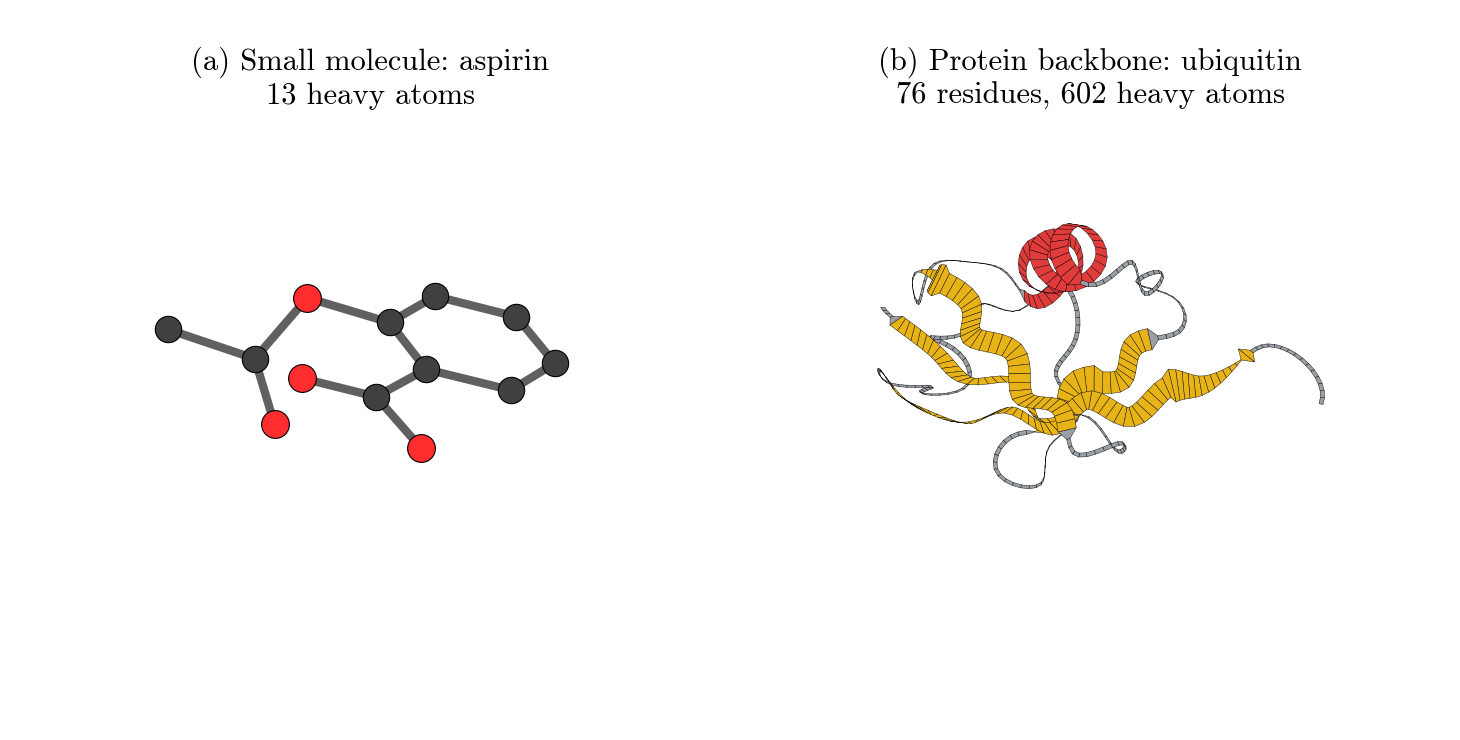
\includegraphics[width=0.9\textwidth]{figures/fig_ch2_domains.png}
\caption{The two molecular domains, at very different scales. (a) A small molecule, aspirin: 13 heavy atoms. (b) A protein backbone, ubiquitin: 76 residues, 602 heavy atoms.}
\label{fig:domains}
\end{figure}
